\usetikzlibrary{arrows.meta,calc}
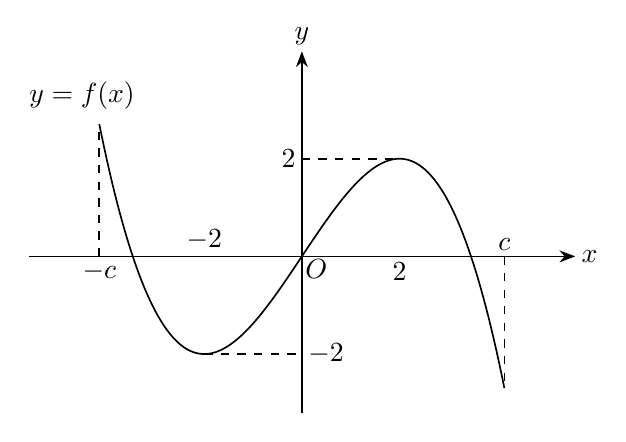
\begin{tikzpicture}[x=0.62cm,y=0.62cm,line width=.6pt,>=Stealth]
\draw[->] (-5.6,0)--(5.6,0) node[right,inner sep=0pt,xshift=2pt]{$x$};
\draw[->] (0,-3.2)--(0,4.2) node[above,inner sep=0pt,yshift=2pt]{$y$};
\node[below right,inner sep=0pt,xshift=1pt,yshift=-1pt] at (0,0) {$O$};
\draw[dashed] (-4.15,0)--(-4.15,2.709);
\draw[dashed] (4.15,0)--(4.15,-2.709);
\draw[dashed] (0,2)--(2,2);
\draw[dashed] (-2,-2)--(0,-2);
\draw[domain=-4.15:4.15,samples=220,smooth] plot(\x,{1.5*\x-pow(\x,3)/8});
\node[left,inner sep=0pt,xshift=-2pt] at (0,2) {$2$};
\node[right,inner sep=0pt,xshift=2pt] at (0,-2) {$-2$};
\node[above,inner sep=0pt,yshift=2pt] at (-2,0) {$-2$};
\node[below,inner sep=0pt,yshift=-2pt] at (2,0) {$2$};
\node[above,inner sep=0pt,yshift=2pt] at (4.15,0) {$c$};
\node[below,inner sep=0pt,yshift=-2pt] at (-4.15,0) {$-c$};
\node[anchor=west,inner sep=0pt] at (-5.6,3.3) {$y=f(x)$};
\end{tikzpicture}
